% !TEX spellcheck = nl_NL
\chapter{Organisatie} \label{hoofdstuk:organisatie}
Tijdens het ontwikkelen van de eerste versie van Canvas.hs is er samengewerkt volgens een paar vooraf geselecteerde methoden. Zo zijn er onderdelen van de Scrum projectmanagement methode toegepast voor een goede planning en duidelijke afspraken. Lees hier meer over in de volgende sectie—\halfref{sec:scrum}.

Bij het ontwikkelen van software is het naast een goede projectorganisatie ook zaak dat er door ontwikkelaars goed samengewerkt kan worden op technisch vlak. Daarbij is het elkaar controlleren en elkaar niet in de weg zitten een belangrijk onderdeel. Hoe dit tijdens de ontwikkeling van Canvas.hs georganiseerd is kan gelezen worden in \fullref{sec:technische_organisatie}.

\section{Scrum} \label{sec:scrum}
Zaken als planning, verdeling van de verantwoordelijkheden en het beslissen over architecturele vraagstukken zijn belangrijk. Om er voor te zorgen dat alle betrokkenen hierover op een gelijke manier denken is er voor het toepassen van een projectorganisatie methode gekozen. Een populaire methode voor software projecten is Scrum. Er is dan ook gewerkt met een variant hiervan tijdens de ontwikkeling van Canvas.hs.

Verschillende rollen zijn toegewezen aan de betrokken personen. Elke samenkomst zijn er zogenaamde scrum besprekingen gehouden en bij aanvang van een nieuwe fase zijn er sprint besprekingen gehouden. Daarbij zijn elke keer opnieuw het project– en sprintbacklog samengesteld en bijgewerkt.

\subsubsection{Rollen}
Er is een verdeling van verantwoordelijkheden gemaakt. Hieronder een kort overzicht van de teamleden en verantwoordelijkheden.
\begin{enumerate}
    \item \emph{J. van Doorn} had de taak van \emph{scrum master} en was verantwoordelijk voor het testen van de software.
    \item \emph{P.T. Jager} was notulist voor alle besprekingen en samen met Buit verantwoordelijk voor de Haskell code.
    \item \emph{L.J. Buit} was verantwoordelijk voor het protocol en samen met Jager verantwoordelijk voor de Haskell code.
    \item \emph{M.J. Roo} was samen met Scheepers verantwoordelijk voor de JavaScript code.
    \item \emph{M.J. Scheepers} was verantwoordelijk voor de gebruiksvriendelijkheid uiteindelijke API en samen met Roo verantwoordelijk voor de JavaScript code.
\end{enumerate}
Naast de teamleden nam de opdrachtgever de rol van \emph{product owner} aan. Hiermee is de opdrachtgever onder andere verantwoordelijk voor het aangeven van de volgorde waarin features ge\"implementeerd.

\subsubsection{Taken}
Taken worden bijgehouden in de zogenaamde \emph{backlogs}. Er is een \emph{backlog} voor alle taken die nog uitgevoegd moeten worden en er is een \emph{backlog} voor de taken die ingepland zijn voor de huidige fase. Taken bestaan uit: projecttaken, als het bijhouden van de planning; ontwikkeltaken, als het oplossen van bugs en het schrijven van nieuwe features; schrijftaken en overige taken.

\begin{figure}[H]
\begin{center}
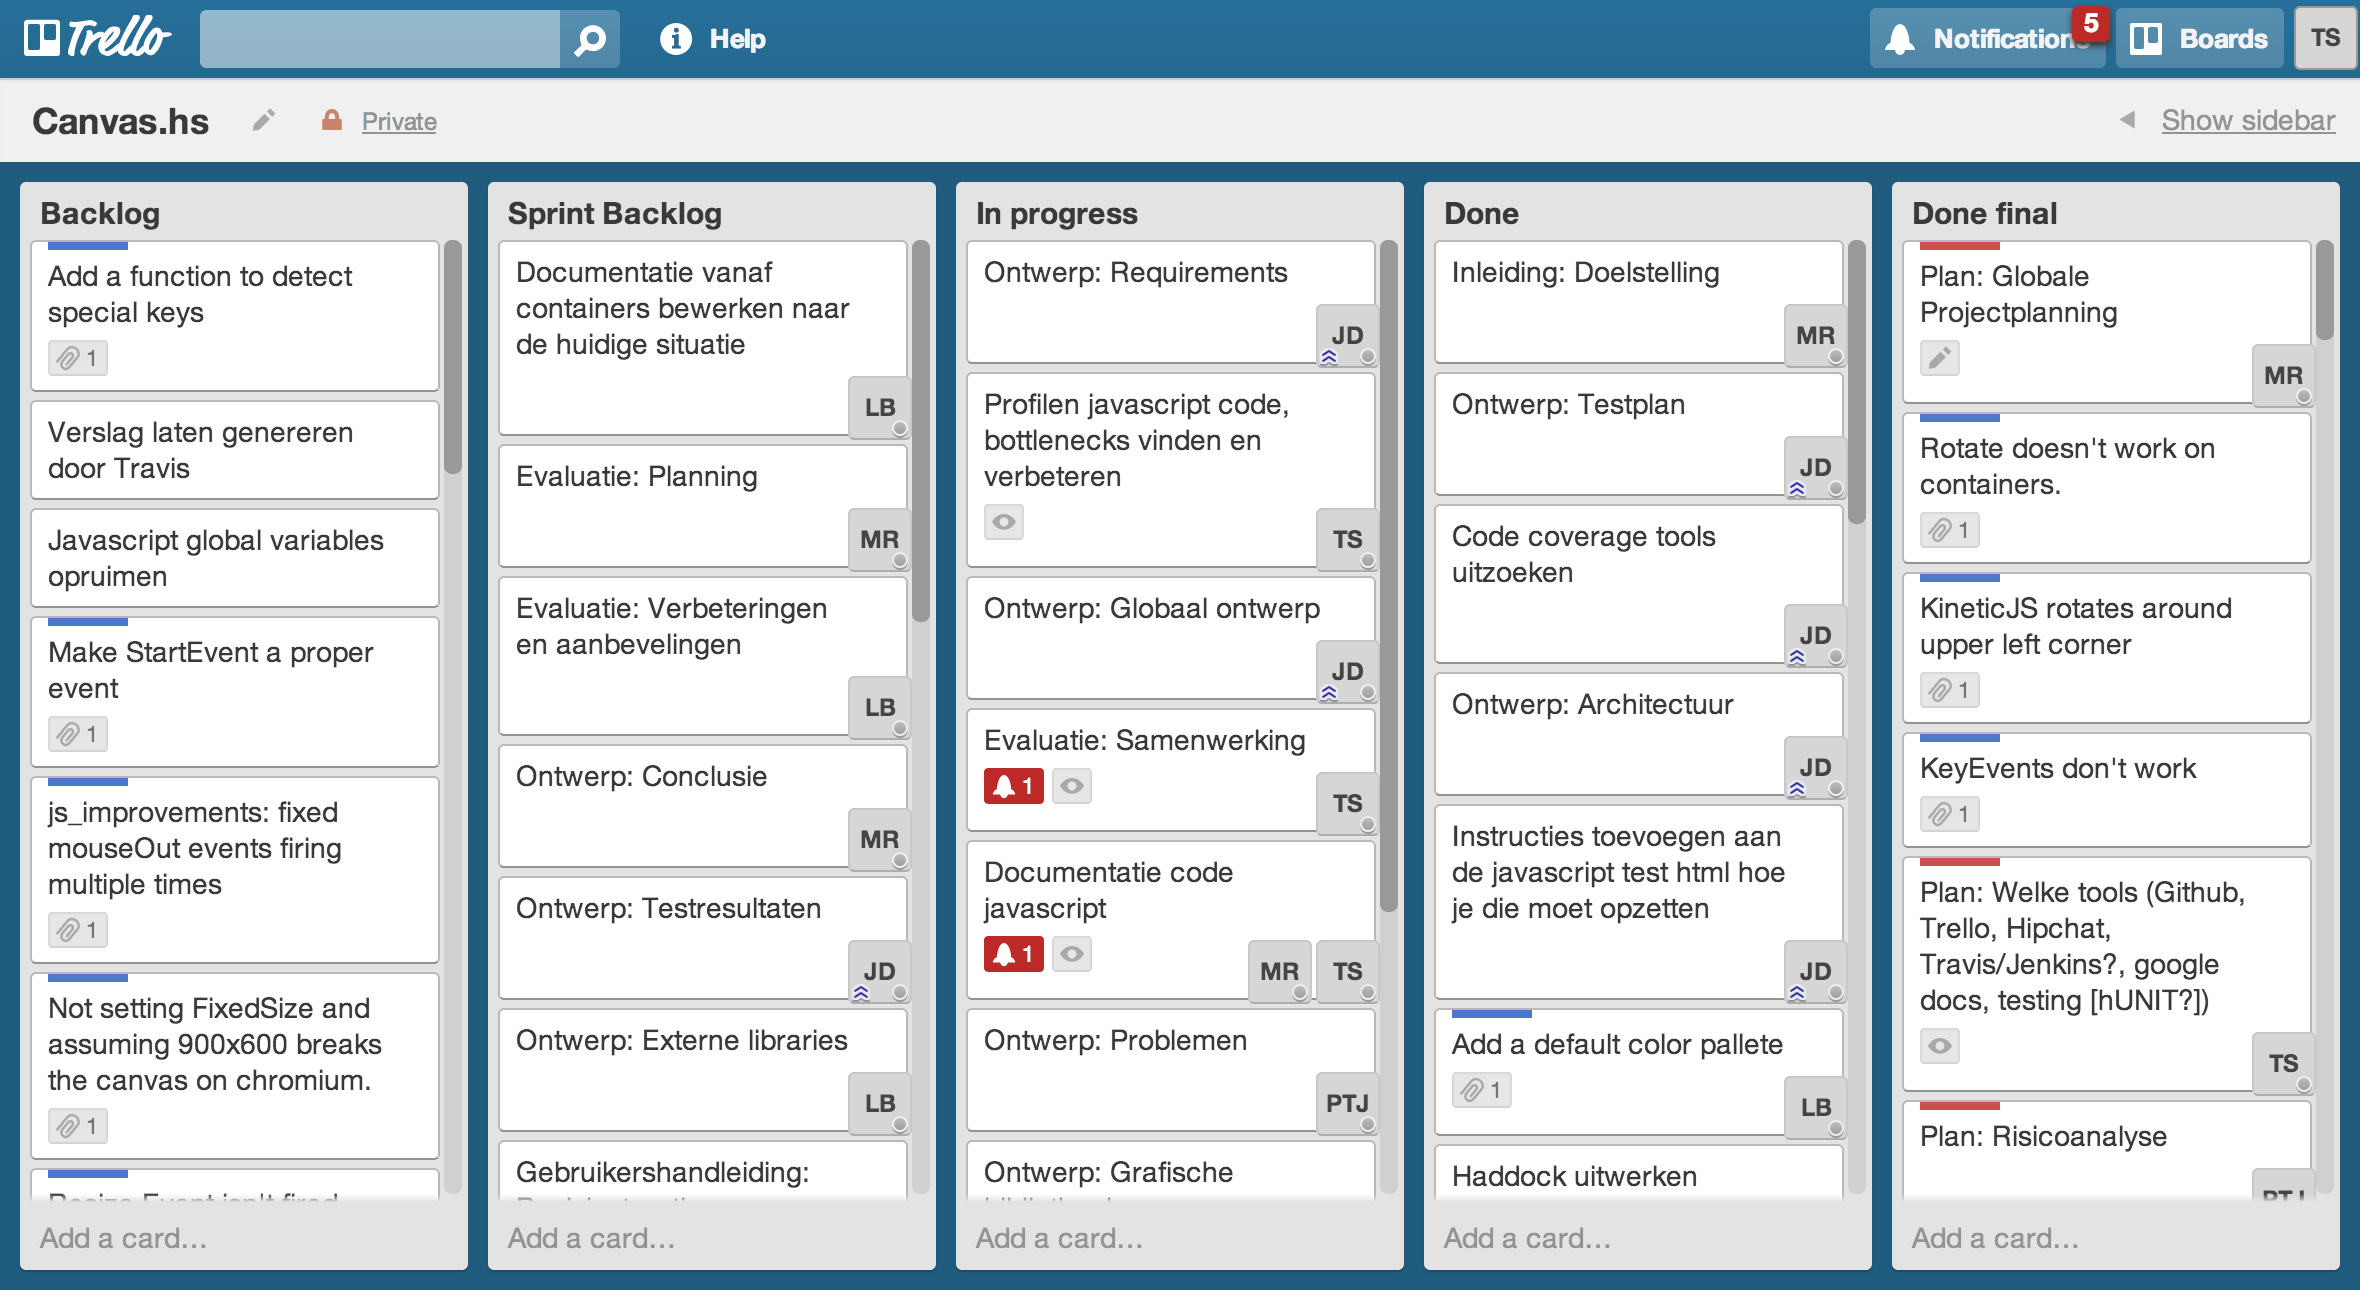
\includegraphics[keepaspectratio,width=\textwidth]{./images/trello.png}
\caption{Trello board}
\label{fig:trello}
\end{center}
\end{figure}

De lijst van ontwikkeltaken werd bijgehouden op het \emph{GitHub} platform—hierover meer in \fullref{sec:technische_organisatie}. Deze ontwikkeltaken werden daar ook wel \emph{issues} genoemd. Ontwikkeltaken en andere taken werd gezamenlijk bijgehouden op \emph{Trello}. Met deze applicatie kan een online takenbord gemaakt worden. De taken werden in de applicatie verdeeld over de verschillende backlogs. In \autoref{fig:trello} is te zien welke status een taak heeft aan de kolom waar deze in staat. Door het gebruik van Trello hebben alle betrokkenen een goed inzicht in de taken die nog openstaan en reeds zijn uitgevoerd.

\subsubsection{Besprekingen}
Er zijn twee typen besprekingen die regelmatig gehouden worden. Ten eerste wordt elke samenkomst de \emph{Scrum bespreking} gehouden. Tijdens deze bespreking vertelt ieder teamlid kort wat hij/zij sinds de vorige bespreking gedaan heeft en of er problemen waren. Daarna verteldt het teamlid waar hij/zij na de bespreking mee bezig gaat. Het is hier de bedoeling dat ieder teamlid een concreet kortetermijn doel stelt.
Ten tweede wordt er bij aanvang van een nieuwe fase een planning gemaakt op basis van de taken in het \emph{project backlog}. De prioriteit per taak wordt aangegeven door de \emph{product owner}, in ons geval de opdrachgever. De teamleden bepalen vervolgens tijdens de bespreking hoeveel van deze taken uitgevoerd kunnen worden en verplaatsen deze naar het \emph{spring backlog}. 

\section{Technische organisatie} \label{sec:technische_organisatie}
Bij het bouwen van software met een groep is het belangrijk dat elke ontwikkelaar zich kan concentreren op de feature die hij/zij aan het ontwikkelen is. Idealiter hoeft er geen rekening gehouden te worden met andere features die door anderen ontwikkeld worden. Er is dan ook gekozen om gebruik te maken van het gedistribueerde versiebeheer systeem \emph{Git} met een centraal repository op \emph{GitHub}.

Er zijn afspraken gemaakt hoe deze versiebeheer software gebuikt moet worden. Zo is er gebruik gemaakt van het \emph{branching model} Gitflow\cite{Gitflow2010}. Als een bepaalde versie van de software op een bepaalde branch staat zegt dit iets over de status van die versie. Zo kan er begonnen worden aan een nieuwe feature vanaf de \inlinecode{dev} branch. En is een versie op de \inlinecode{master} branch klaar voor gebruik. Het insturen van een nieuwe versie wordt ook wel een \emph{commit} genoemd.

\begin{figure}[H]
\begin{center}
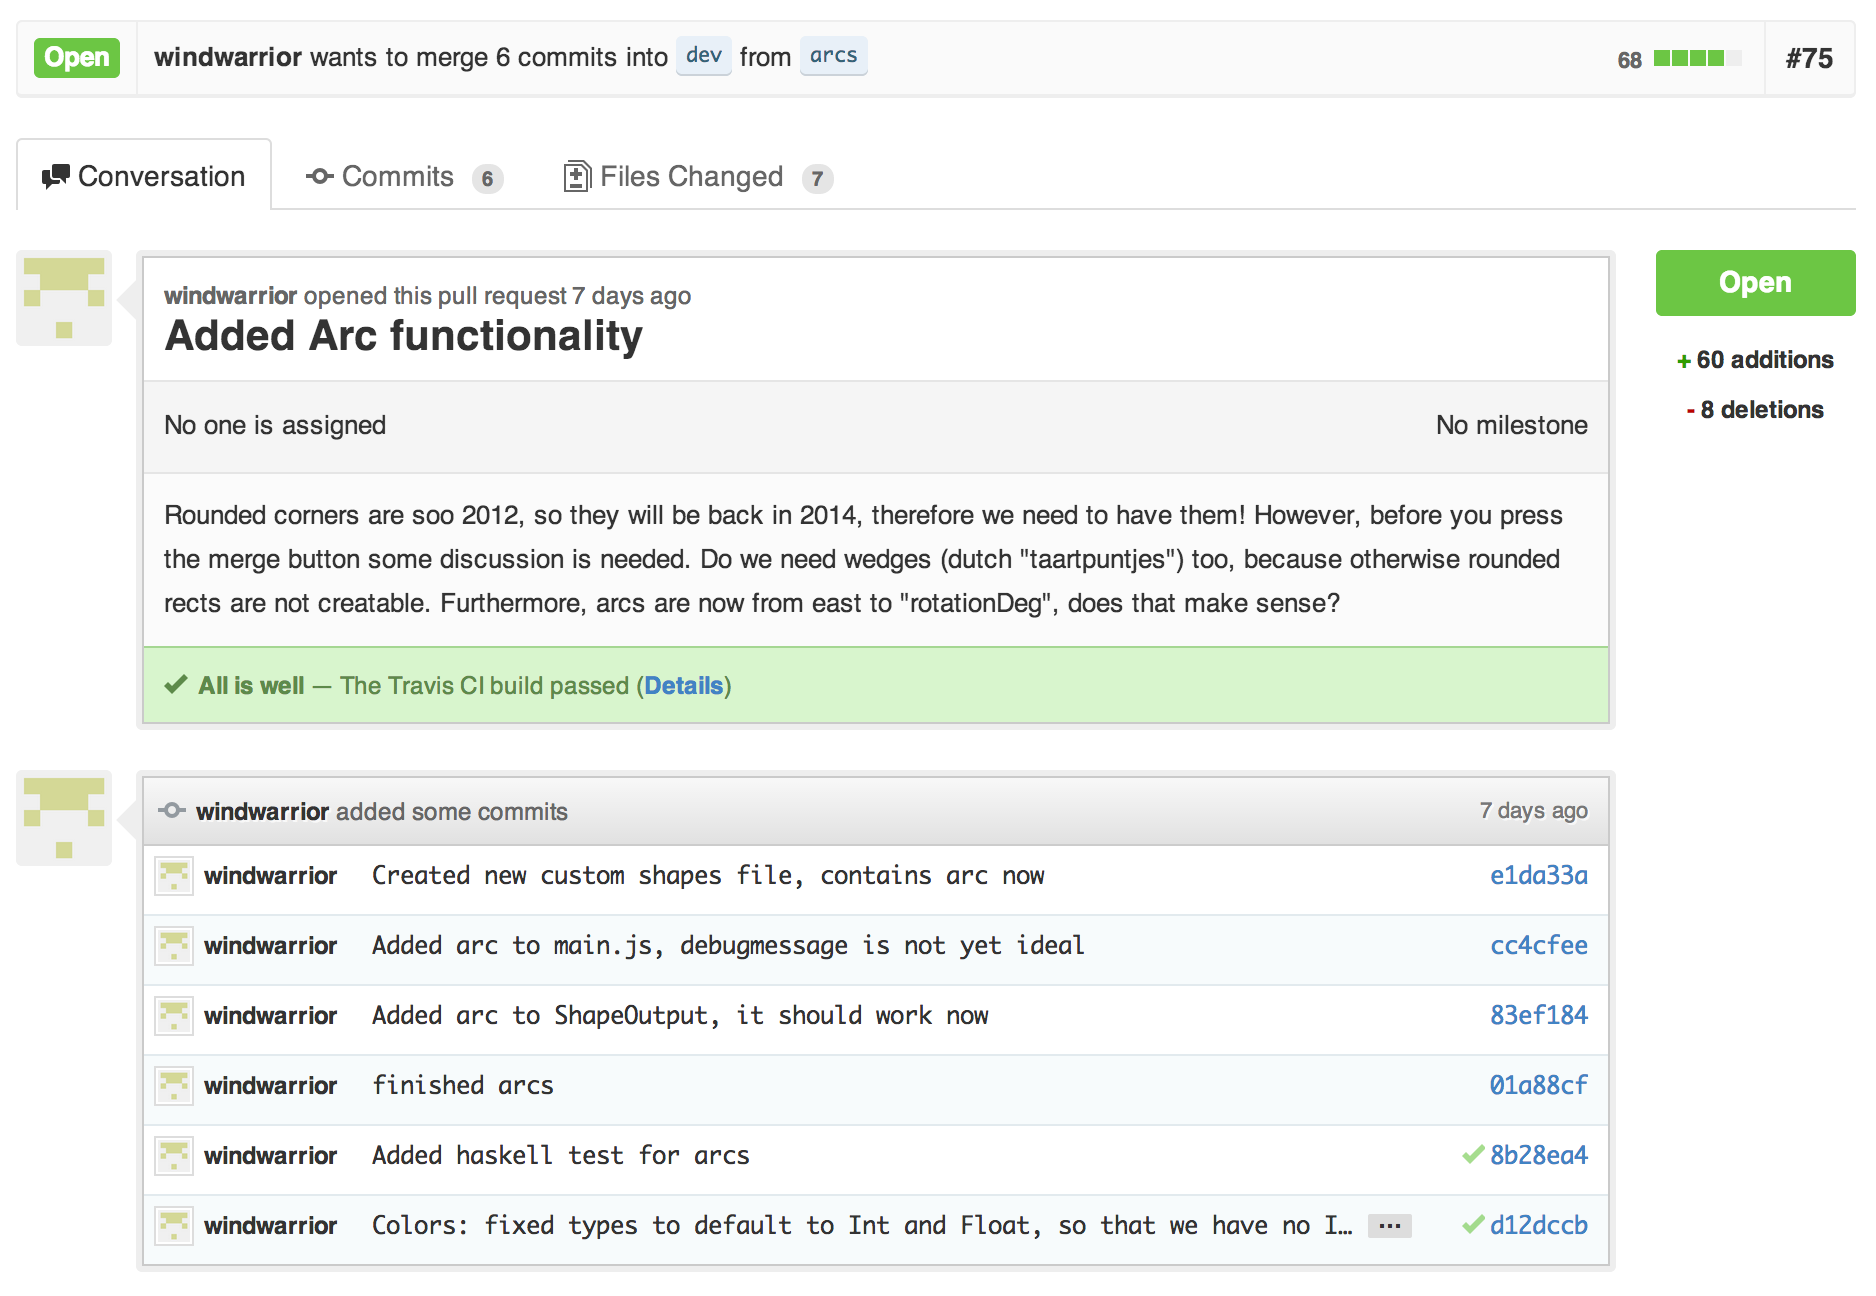
\includegraphics[keepaspectratio,width=\textwidth]{./images/pullrequest.png}
\caption{Pull Request \#75 Arcs geimplementeerd. – \url{https://github.com/CanvasHS/Canvas.hs/pull/75}}
\label{fig:pullrequest}
\end{center}
\end{figure}

\subsubsection{Pull requests}
Bij aanvang van de ontwikkeling van een nieuwe feature wordt er een nieuwe branch gemaakt vanaf de \inlinecode{dev} branch. Een voorbeeld hiervan is de \inlinecode{arcs} branch. In \fullref{sec:shapesext} staat beschreven hoe \inlinecode{Arc} shapes toegevoegd kunnen worden. Dit is gebeurd op een aparte branch die begonnen is vanaf de \inlinecode{dev} branch, zie \autoref{fig:pullrequest}.

Als een feature af is moet deze beoordeeld door een ander teamlid voordat de feature samengevoegd kan worden met de \inlinecode{dev} branch. Om dit te bewerkstelligen wordt gebruik gemaakt van een \emph{pull request}. Deze pull request bevat informatie over de wijzigingen tenopzichte van de versie die op de \inlinecode{dev} branch staat. Een beoordelaar kan de code lezen en deze goedkeuren. Op het moment dat de code goed wordt gekeurd komt een nieuwe versie met de nieuwe feature op de \inlinecode{dev} branch te staan.

\subsubsection{Continuous integration met Travis CI}
Om het beoordelen van code gemakkelijk te maken is er gebruik gemaakt van de \emph{continuous integration} software \emph{Travis CI}. Deze software luistert naar nieuwe commits naar het centrale repository, na het insturen van een nieuwe versie naar het centrale repository wordt er door Travis CI een virtuele machine opgestart. Deze machine download de zojuist ingestuurde versie en compileert deze inclusief alle tests middels het uitvoeren van een \emph{buildscript}. Dit buildscript staat in de root directory van het repository. Als het compileren slagen en alle tests slagen ook zal de build als geslaagd worden gemarkeerd, zie \autoref{fig:pullrequest} voor het resultaat van de laaste commit op de \inlinecode{arcs} branch. Mocht één van de tests niet slagen of het compileren niet slagen wordt de build als mislukt gemarkeerd.

\begin{figure}[H]
\begin{center}
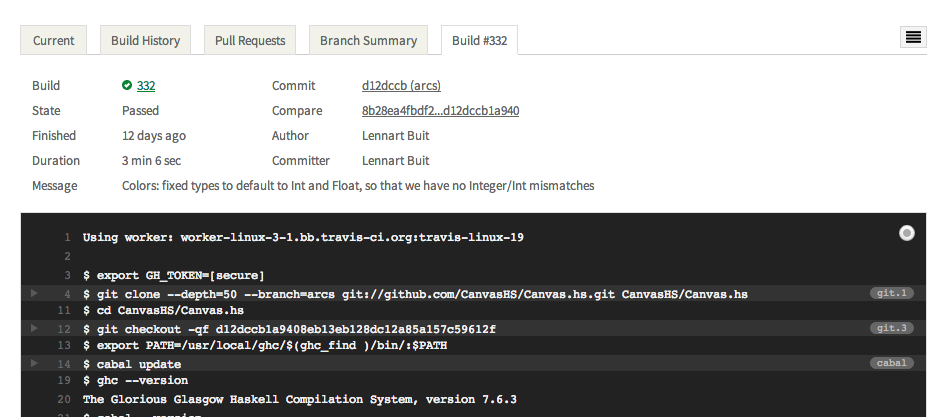
\includegraphics[keepaspectratio,width=\textwidth]{./images/travis.png}
\caption{Build van Pull Request \#75. – \url{https://travis-ci.org/CanvasHS/Canvas.hs/builds/16168834}}
\label{fig:travis}
\end{center}
\end{figure}

Informatie over het resulstaat van een build kan gebruikt worden bij het boordelen van een pull request. Als een beoordelaar ziet dat de build uit een pull request succesvol is, zoals bijvoorbeeld te zien bij \autoref{fig:pullrequest}, heeft hij/zij een goede indicatie dat de pull request veilig gemerged kan worden.

Het buildscript voert naast de compilatie nog een paar nevenfuncties. Zo genereert het buildscript ook de documentatie en uploadet het buildscript deze naar de Canvas.HS website—\url{http://canvashs.github.io}. Op de website kan de documentatie bekeken worden per build. Hierdoor hoeven ontwikkelaars zelf geen documentatie meer te genereren en hebben zij altijd, up-to-date, en doorzoekbare documentatie.

\section{Conclusie}
Met duidelijke afspraken over project- en technische organisatie is er een basis voor het ontwerpen en ontwikkelen van Canvas.hs. In \autoref{hoofdstuk:evaluatie} kan een evaluatie en reflectie gelezen worden over het toepassen van de, in dit hoofdstuk beschreven, organisatie vormen en technieken. 
